

\subsection{Graph Semantics}\label{semantic}

Deciding the correct semantic representation for a visualisation is often just as important as the selecting the correct syntatic style. Semantic features are often applied post generation \cite{aestheticsgraphvis} and have uses in the encoding of additional information and clarifying any results within the data. As a means of achieving both an aesthetically pleasing outcome, and an easy to understand visualisation, we must first consider what features we, or the reader, are most interested in. Once this has been decided, we begin to explore various methods for representing them. 

\subsubsection{Limitations}

When selecting visualisation semantics, there are several limitations that we must consider. 

\paragraph*{Visual}
When it comes to Visual analytics the greatest bottleneck is due to the resolving power of the eye - this is known as an acutie. Acuities are a measure of the angle of an observed object with the viewer's eye using arcs (one arc equates to $\frac{1}{60}^{th}$ of a degree). This provides a unit of measurement for the total amount of information density we can feasibly perceive, \cite{ware}. 

 In ophthalmology there exist four types of  acuities: 
\begin{itemize}
\item[-] \textbf{detection}: The smallest size an object can be whist still being seen
\item[-] \textbf{recognition}: The smallest size an object can be to be recognised
\item[-] \textbf{resolution}: The smallest distance between two objects before they begin to merge
\item[-] \textbf{localization}: The smallest amount of visual change that can be measured between two objects
\end{itemize}

These provide a set of considerations which may be used to assess a visualisation. Depending on what encoding we use, it is possible to improve/hinder the readers ability to percieve information, \autoref{acuity}. An example of this would be that for a Macbook Pro retina screen\footnote{A retina screen, is half the maximum possible resolution of the human eye at a 30cm distance. Additionally the operating system interpolates in sets of 4 pixels, such that the image displayed may not be at full resolution.}, where at 87 pixels/cm\footnote{at 57cm from the screen} we can display at most 2 million resolvable nodes. If we wished to add links between nodes, the total resolvable items is reduced to one million
\cite{ch10}. 

\begin{figure}[H]
\begin{center}
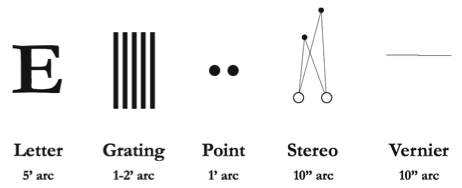
\includegraphics[scale=.6]{figures_c1/acuity.png}
\end{center}
\caption{Important acuities in visualisation, Source: \cite{ch10,ware}}\label{acuity}
\end{figure}


\paragraph*{Cognitive}
Although it may be possible to distinguish 1 million nodes and links visually, interpreting and understanding these presents another problem. The visual thinking laboratories, \cite{vt}, have a range of publications exploring how presentation can improve though, cognition and communication between info-graphic and reader. \cite{OpenVis}, explains that the time required to interpret a visualisation is directly related to the encoding used to hi-light the data within it. Also problems of `intentional blindness' and misinterpretation are problems which are often occurred with poorly thought out encodings.  

In considering the cognitive load of a visualisation, \cite{emotional} provides a list of three categories which should be explored:


\begin{itemize}
\item[1.] Firstly we have the visceral level, a subconscious process where decisions are made rapidly based on sensory inputs to the body. 
This is usually due to our inherent ability to locate patterns and changes due to semantic properties which shift the focus of the user.  

\item[2.] Next follows the behavioural level (mostly subconscious). These are often learn reaction to changes noted as part of the visceral level. Here reactions may be honed on and influenced by past experiences and events. 

\item[3.] Finally we reach the reflective level. Here the user collates all sensory input from the previous two levels and makes an informed conclusion about the underlying data. Conclusions drawn here can be used to bias the methods used within the behavioural level in future events. 
\end{itemize}

\paragraph*{Technological}
In addition to human limitations, there may be restrictions due to the medium a visualisation is created/presented on. In addition to monitor resolution issue earlier, much scientific research is constrained by the size, resolution and colour quality of the presentation mediums used for talks, printing or posters. \cite{ware} explains that a printer capable of producing 1200 dots per inch squared, can only do this for black/white binary images. If for instance 256-greyscale is used, the resulting resolution is then at-least 10 times smaller. This is because printers a Monet style approach to create shading and colour. It therefore follows that at full CYMK, the output resolution will be worse. 

It is also important to have a graph fitting the same overall shape of the canvas on which it is presented, \cite{graphmetnew}. This not only makes optimal use of any space available, but also reduces the visual complexity as it minimises the number of distinct shapes available to the user. 




 




\subsubsection{Node Encoding}
Within a graph, the nodes represent the set of items we are exploring. Each of these often contain a multitude of features and properties relating directly to them, be it the user details for a retail/fraud network, or the chemical composition and concentration of a species in the MCM. Features of a node describe and additional properties and may be used to determine its interaction with other nodes\footnote{This is further explored in Chapter 4}, \cite{protocol}. It is for this reason that graph convoluted neural networks, \cite{t2gcn}, require a  `feature matrix' describing each node, in addition to the network structure and edge weightings. Within a visualisation, a node may be represented in a range of ways. 

\paragraph*{\color{c4}Circle attributes}



The simplest of these range from the use of colour, shape, size, thickness and stroke (outline) to indicate a group. Here it is possible to provide information such as a species concentration based on its size, its importance with its colour, its degree with its opacity and its category with its stroke colour \cite{brightness,colour}. Such descisions depend on what properties you are trying to show. For instance red species in \autoref{fig:nodestyle} are primary emitted VOCs, orange species exist between both the MCM and the CRI (see figure caption) mechanism, and blue ones are lumped species which do not appear as part of the MCM.  


\paragraph*{\color{c1}Chemical Structure}
Traditional chemical diagrams use the chemical structure to depict the types of reaction that occur , \autoref{fig:butane}. This make it intuitive to extract information about functional group and bond changes within species. Such a method of representation, is indeed useful, however when visualising hundreds, if not thousands of nodes on a page, it results in occulsion, or labels too small to resolve visually. 

\paragraph*{\color{c2}Species Name}

Much like the chemical structure, a species name is proven useful in explaining to the user its chemical properties (often due to prior knowledge, or the ability to look this up). Unfortunately since names have differing lengths, this can cause problems, especially with large numbers of closely located nodes. A solution to this may be to adjust the font size to fit in within the circle radius of the node. However this does come with its problems - for instance very small nodes may have text smaller than a pixel, or the misleading notion that longer names are less important, since they are represented by a smaller font. 


\paragraph*{\color{c3}Interactivity}

Ben Shneiderman's famous mantra goes: \emph{`overview first, zoom and filter, details on demand'} \\ \cite{mantra}. This goes hand in hand with the philosophy used within the design of an interactive visualisation.

For complicated systems, interactivity plays a vital role in unraveling complexity and reducing clutter \cite{interaction1}. It allows the user to actively query only the items that they are interested in whilst still displaying all the information in a single location \cite{oneplace}. 

A comprehensive list of all available interaction types and styles are provided in \cite{ch6}. Some examples of interaction are:\\ 

\begin{table}[h]
    \centering
    \begin{tabular}{p{.45\textwidth}p{.45\textwidth}}
\textbf{Hi-lighting}
\begin{itemize}
\item Hovering
\item Brushing and Linking
\item Magic Lenses (see hidden objects)
\end{itemize}
&
\textbf{Visual Structure-Level Interaction}
\begin{itemize}
\item Selection
\item Changing layout/mapping attributes
\item Changing representation
\end{itemize}
\\
\textbf{Navigation}
\begin{itemize}
\item Pan / Zoom
\item View Distortion (fisheye)
\end{itemize}
&
\textbf{Data Level Interactions}
\begin{itemize}
\item Adding / Filtering
\item Search / Query
\end{itemize}

\end{tabular}
    \caption{\textbf{A selection of interactive methods.}}
    \label{tab:interactive}
\end{table}

\begin{figure}[H]
     \centering
     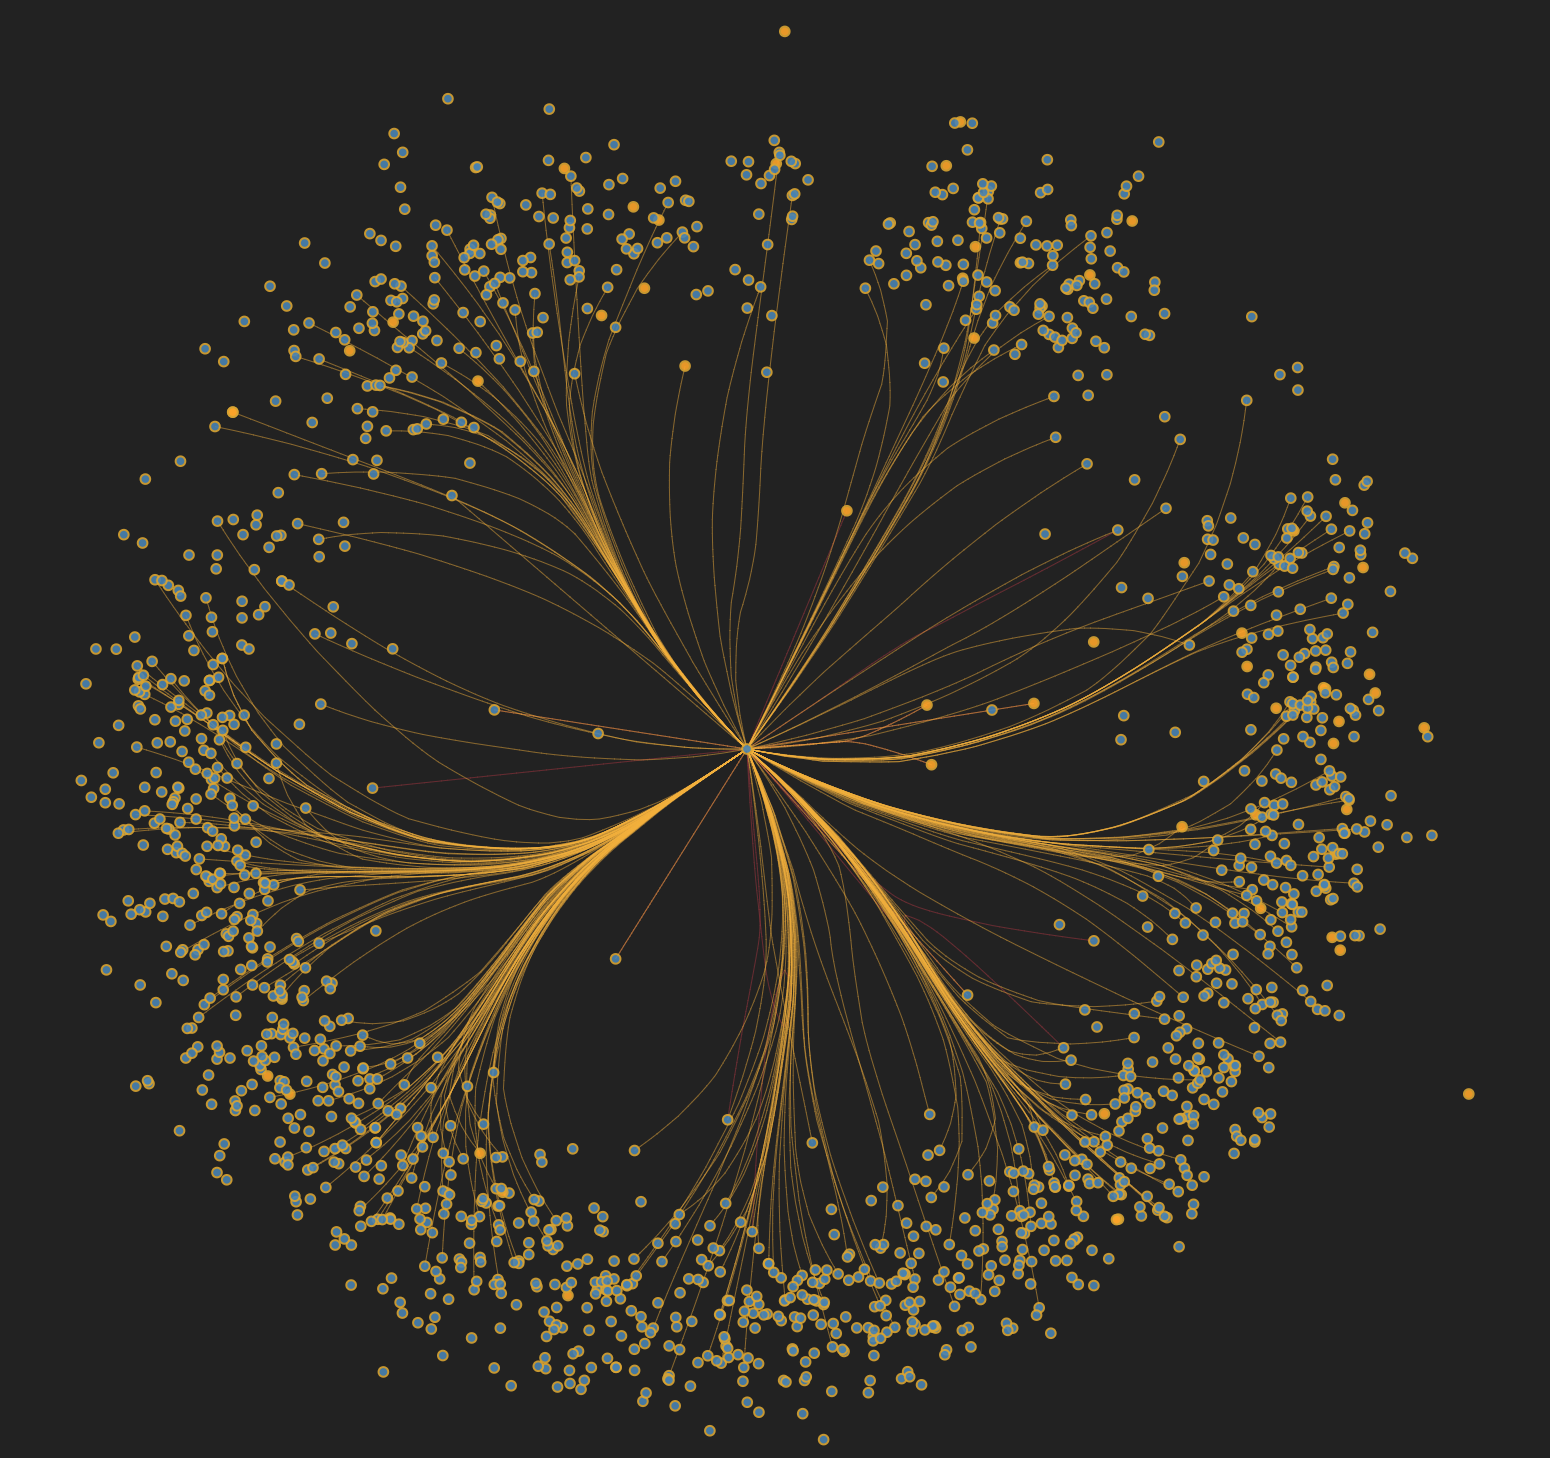
\includegraphics[width=0.7\textwidth]{figures_c1/layout/CObranches.png}
        \caption{\textbf{Using mouseover edge-selection to hilight all links related to a node. } This figure shows how in using interactivity it is possible to reduce clutter and filter the information presented by a densely populated graph. In this case the mercator projection (\autoref{sec:merc}) is used, with reactions relating to Carbon Monoxide (centre) hilighted. Orange lines represent reactions producing CO whist the red (some of which may be hidden) are of reactions with CO.  }
      \label{fig:tooltip}
\end{figure}

\paragraph*{\color{c5}External Labeling}
In cases where interactivity is not possible, such as papers, books and this thesis, an alternative approach to data selection has to be employed. Here nodes which are central to the explanation of a certain point are filtered by the author, and displayed through the use of external labels. It is found that having links at 45 and 90 degree angles (such as in transport maps) lead to a clearer layouts and better distinction from the links already within the graph. Automatically generated labels within the thesis are made using \cite{d3annotate}.



\begin{figure}[H]
     \centering
     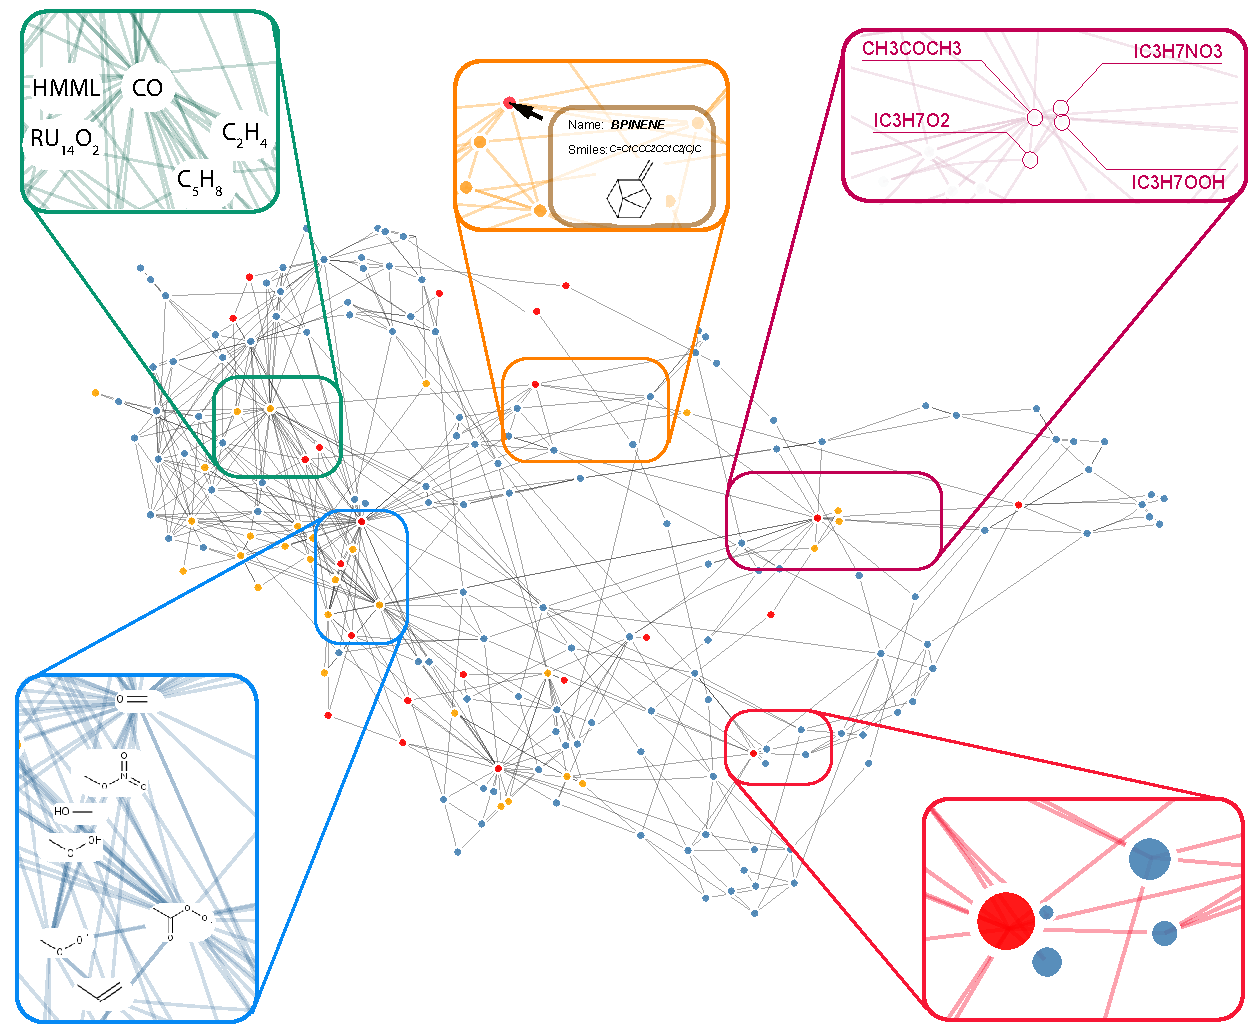
\includegraphics[width=\textwidth]{figures_c1/NODES_001f3d-00775b-ff9000-f71735-c10053.pdf}
        \caption{\textbf{A graph showing 5 different node encoding methods.} These are Circle Atrributes (red), Chemical structure (blue), Species Name (green), External Labels (maroon) and interactive selection (orange). The network shows the Common Representative Intermediate species (CITE) mechanism. Node colours represent primary emitted VOCs (red), MCM species (orange) and lumped CRI-only species (blue).  }
      \label{fig:nodestyle}
\end{figure}







\subsubsection{Edge Properties}


Defining the purpose of graph-energy models as: a means for creating a visualisation from which the viewer can infer properties of the data \cite{noack}, it can be seen that this criterion is easily met in small and sparse graphs. However non-planar examples with high edge density (lots of links) can easily result in tangled results with impractical running times \cite{tvg}. In most cases attaining an optimal solutions here seems to be computationally infeasible \cite{nicelyanneal}. This is generally because graphs primarily focus on hi-lighting a specific purpose or following a set of aesthetic heuristics \cite{eyetrack}. 

Butane model 


\paragraph{Muti-variate edges}
Since there are multiple relationships between species, it is important to decide if simplifying the network would be of benefit. Although it is possible to \autoref{fig:multiedge}.. 
this may cause unecessary clutter for larger networks. Instead it is often useful to simplify the graph, and encode the edge properties within the vector object. This allows the user to retreave any additional information by hovering over the edge or connecting nodes, as required. Should the topic of interest require a specific property, then it would also be possible to remove, or hide, all edges which do not contain it. This produces an interactive graphic containing all the required information, as and when needed, without the unecessary clutter of having every reaction shown. 

\begin{figure}[H]
     \centering
     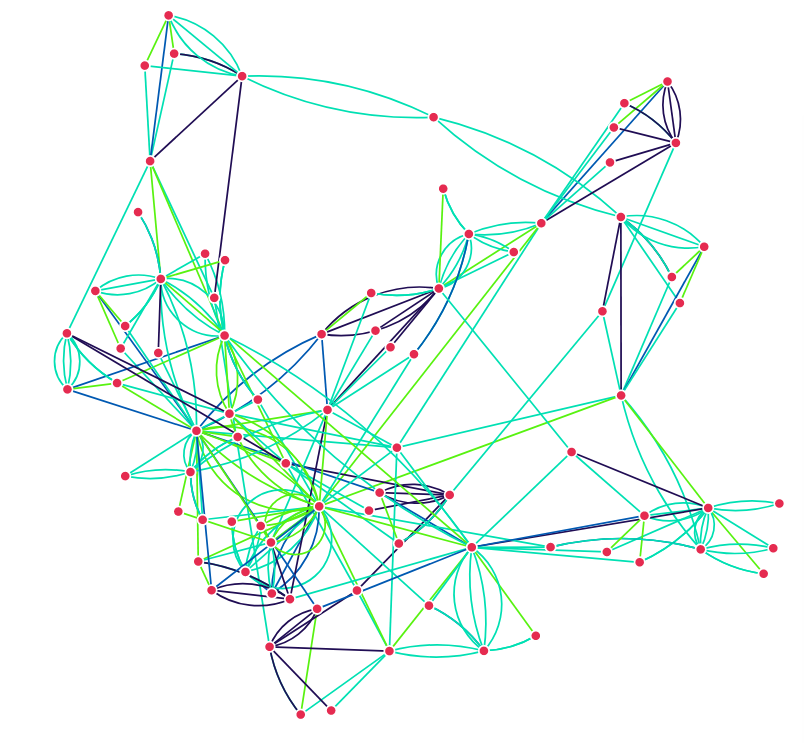
\includegraphics[width=.7\textwidth]{figures_c1/edgetype/multiquadratic.png}
        \caption{\textbf{Multiple edges coloured by type of reaction.} Using the overarching categories of reaction type (see fig wuclan) each type of reaction between two nodes can be visualised using the multi-link format. Photolysis (Bright green), Radical/Other (Amazonite / Teal) Decomposition (Honolulu Blue), RO2(Space Cadet / Purple)}
      \label{fig:multiedge}
\end{figure}

% %
% Photolysis (Bright green), Radical/Other (Amazonite / Teal)
% Decomposition (Honolulu Blue), RO2(Space Cadet / Purple)
% 





\paragraph{Edge Direction}
When using a directional graph it is convention to use arrow heads to represent this. However in high density regions it is often found that arrow heads take up precious real estate in the drawing area \cite{noarredge}. As an alternative, colour and line-type can be used to represent the direction instead. This example can be seen in the routing networks presented by \cite{networkrouting}. One example applicable for chemistry would be the use of dashed lines to represent mono-directional relationships, and continuous lines for bidirectional ones. 








\paragraph{Edge Shape}
Edge shape is important, as it is the medium we use to represent relationships within a graph. For orthogonal graphs, poly-line curved edges are used to provide a layout which is simpler and easier to read \cite{ortho}. For asymetric graph drawings circular Lombardi-style curves and cubic brezier lines have been used to reduce the clutter in high edge-density drawings, \cite{lombardi,bezier}. \autoref{fig:curvededge} shows a selection of different edge types for the Butane MCM subset.The liear network (\autoref{fig:curvededge}a ) consists of straight lines betwen nodes. If a multi-edge graph is required, it is impossible to represent this as all edges between two nodes follow the same path. To improve on this a quadratic arc (\autoref{fig:curvededge} b) can be used. This presents a symmetric representation where each edge is revealed. Finally bezier curves (described below) can be used to show an asymetric representation of the multi-edge graph (\autoref{fig:curvededge}c). Both sets of curved representation rely on a set of control points, allowing the designer to control the curve shape, steepness and asymmetry. 

\paragraph*{Bezier Curves}
Bezier curves are named after Pierre Bezier who used them in the bodywork design of Renault cars in the 1960s \cite{beziermath}. Since then they have been widely used in graphs,computer graphics, font design and animation/interactivity response \cite{bezier,beziermath,beziercomputer}. Bezier curves come in a range of possible dimensions, cubic beziers are the most commonly used within network visualisation. These contain four control points respectively which can be used to determine the shallowness of the curve through design. In general relatively shallow curves are prefered, as these do not introduce unecessary edge crossing or abrupt changes, which have been shown to hinder a users ability to isolate items of interest, \cite{ch6graphredability}.


\begin{figure}[H]
     \centering
      \begin{subfigure}[b]{.32\textheight}
         \centering
     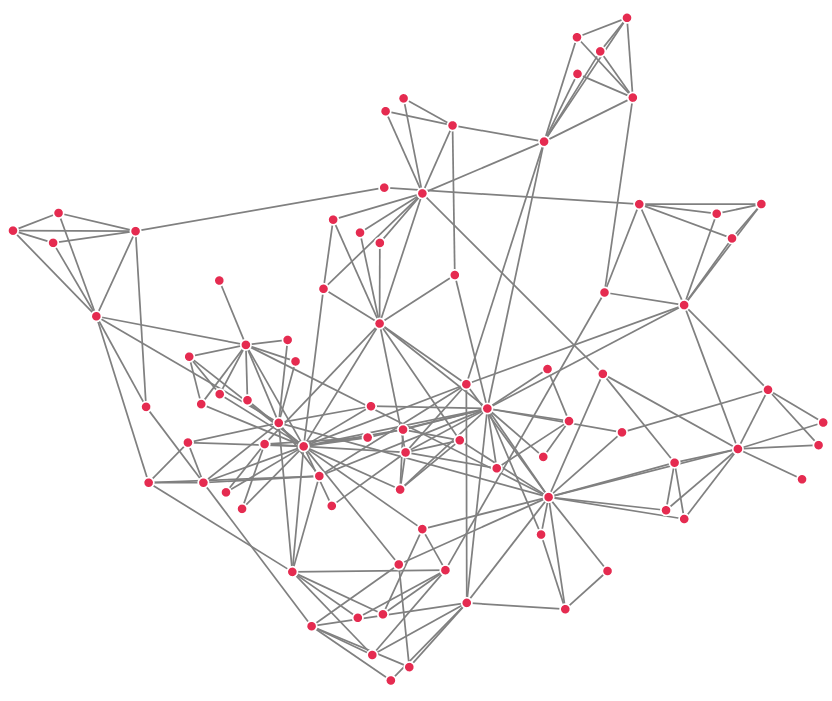
\includegraphics[width=\textwidth]{figures_c1/edgetype/linearsingle.png} \caption{Linear (single-edge)}
     \end{subfigure}\\
    \begin{subfigure}[b]{.32\textheight}
         \centering
     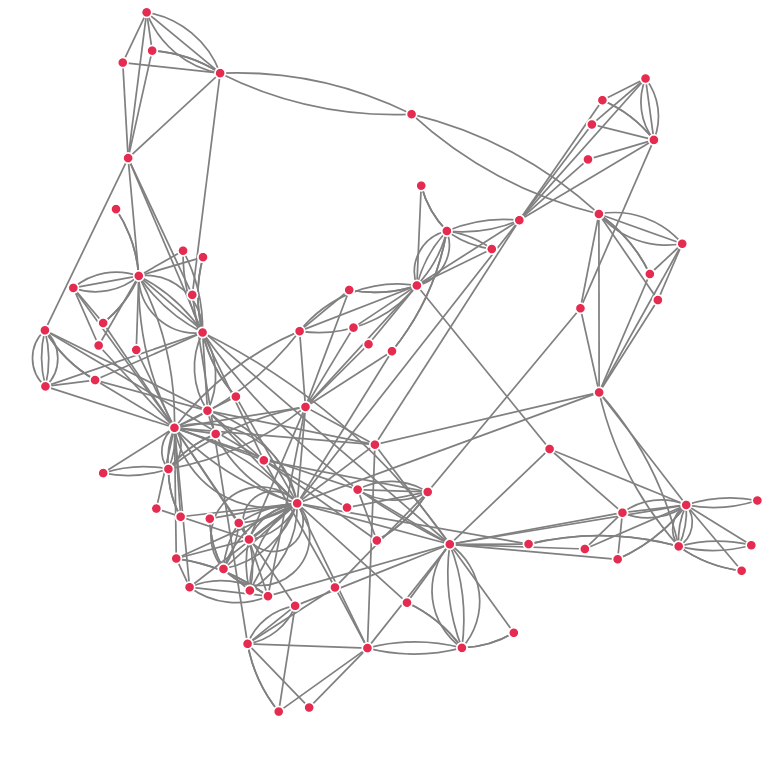
\includegraphics[width=\textwidth]{figures_c1/edgetype/multiquadraticgray.png}
     \caption{Quadratic (multi-edge)}
     \end{subfigure}\\
     \begin{subfigure}[b]{.32\textheight}
         \centering
     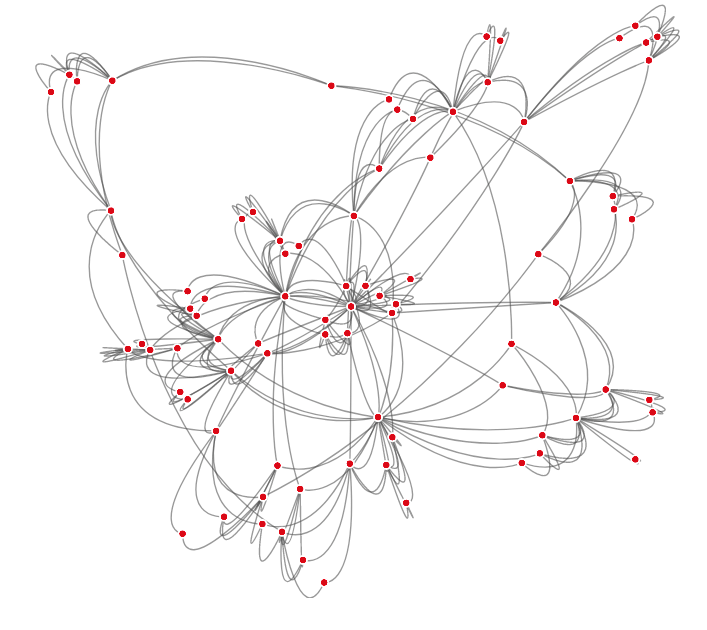
\includegraphics[width=\textwidth]{figures_c1/edgetype/multibeziergray.png}
     \caption{Bezier (multi-edge)}
     \end{subfigure}
        \caption{\textbf{A selection of edge shapes for the butane network.}       }
      \label{fig:curvededge}
\end{figure}








\paragraph{Edge Bundling }
Pioneered by \cite{bundlepioneer}, edge bundling techniques are an effective way to reduce visual clutter. Much like a force graph, edges are represented as a string of lined points. This allows for edges to be pulled together (attracted to one another) and produces a visualisation akin to moving water droplets on a hydrophobic surface. \autoref{fig:edgebundling} shows how in changing the amount of atraction between edges, it is possible to reduce clutter in a visualisation. 


\begin{figure}[H]
     \centering
      \begin{subfigure}[b]{.49\textwidth}
         \centering
     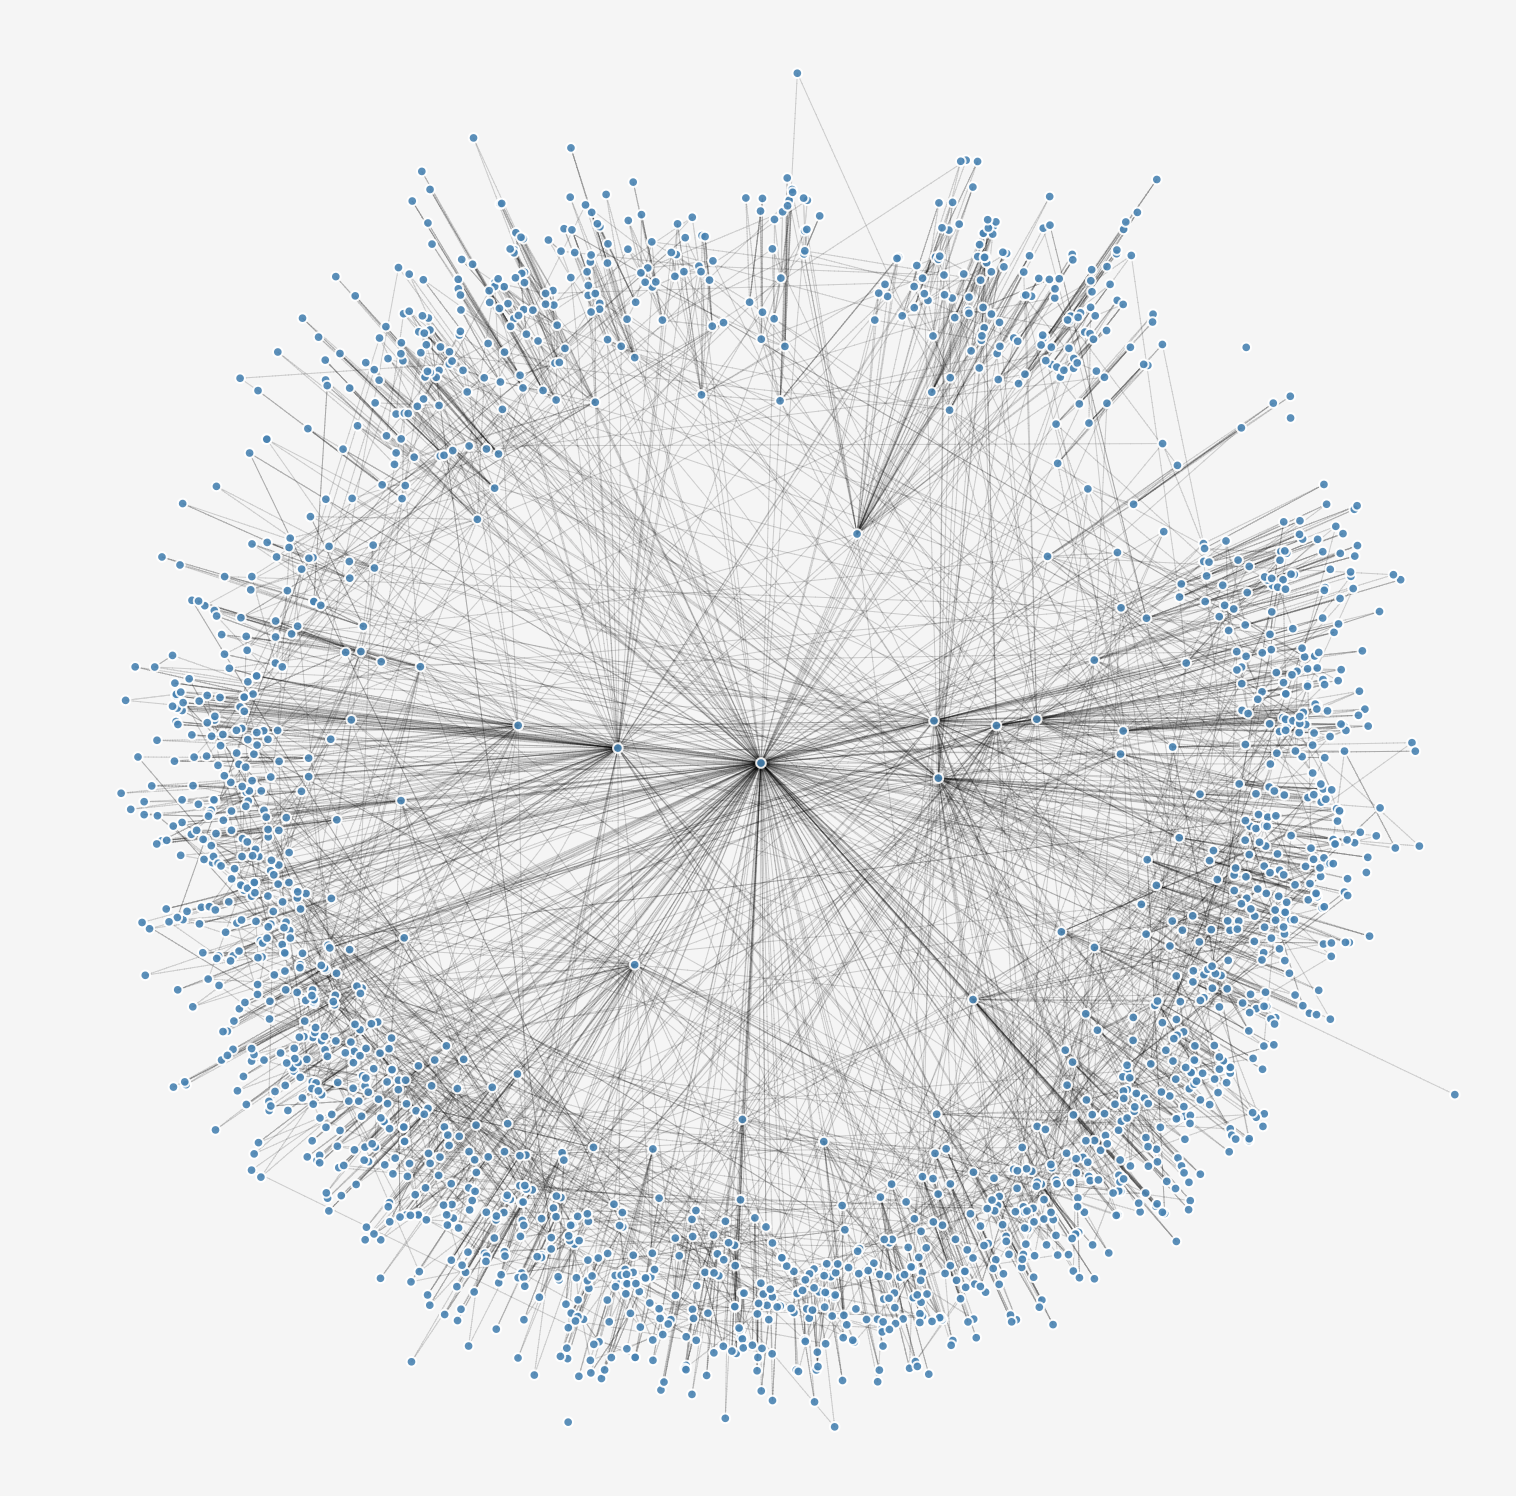
\includegraphics[width=\textwidth]{figures_c1/layout/merc1.png} \caption{$\theta = 1$}
     \end{subfigure}
\begin{subfigure}[b]{.49\textwidth}
         \centering
     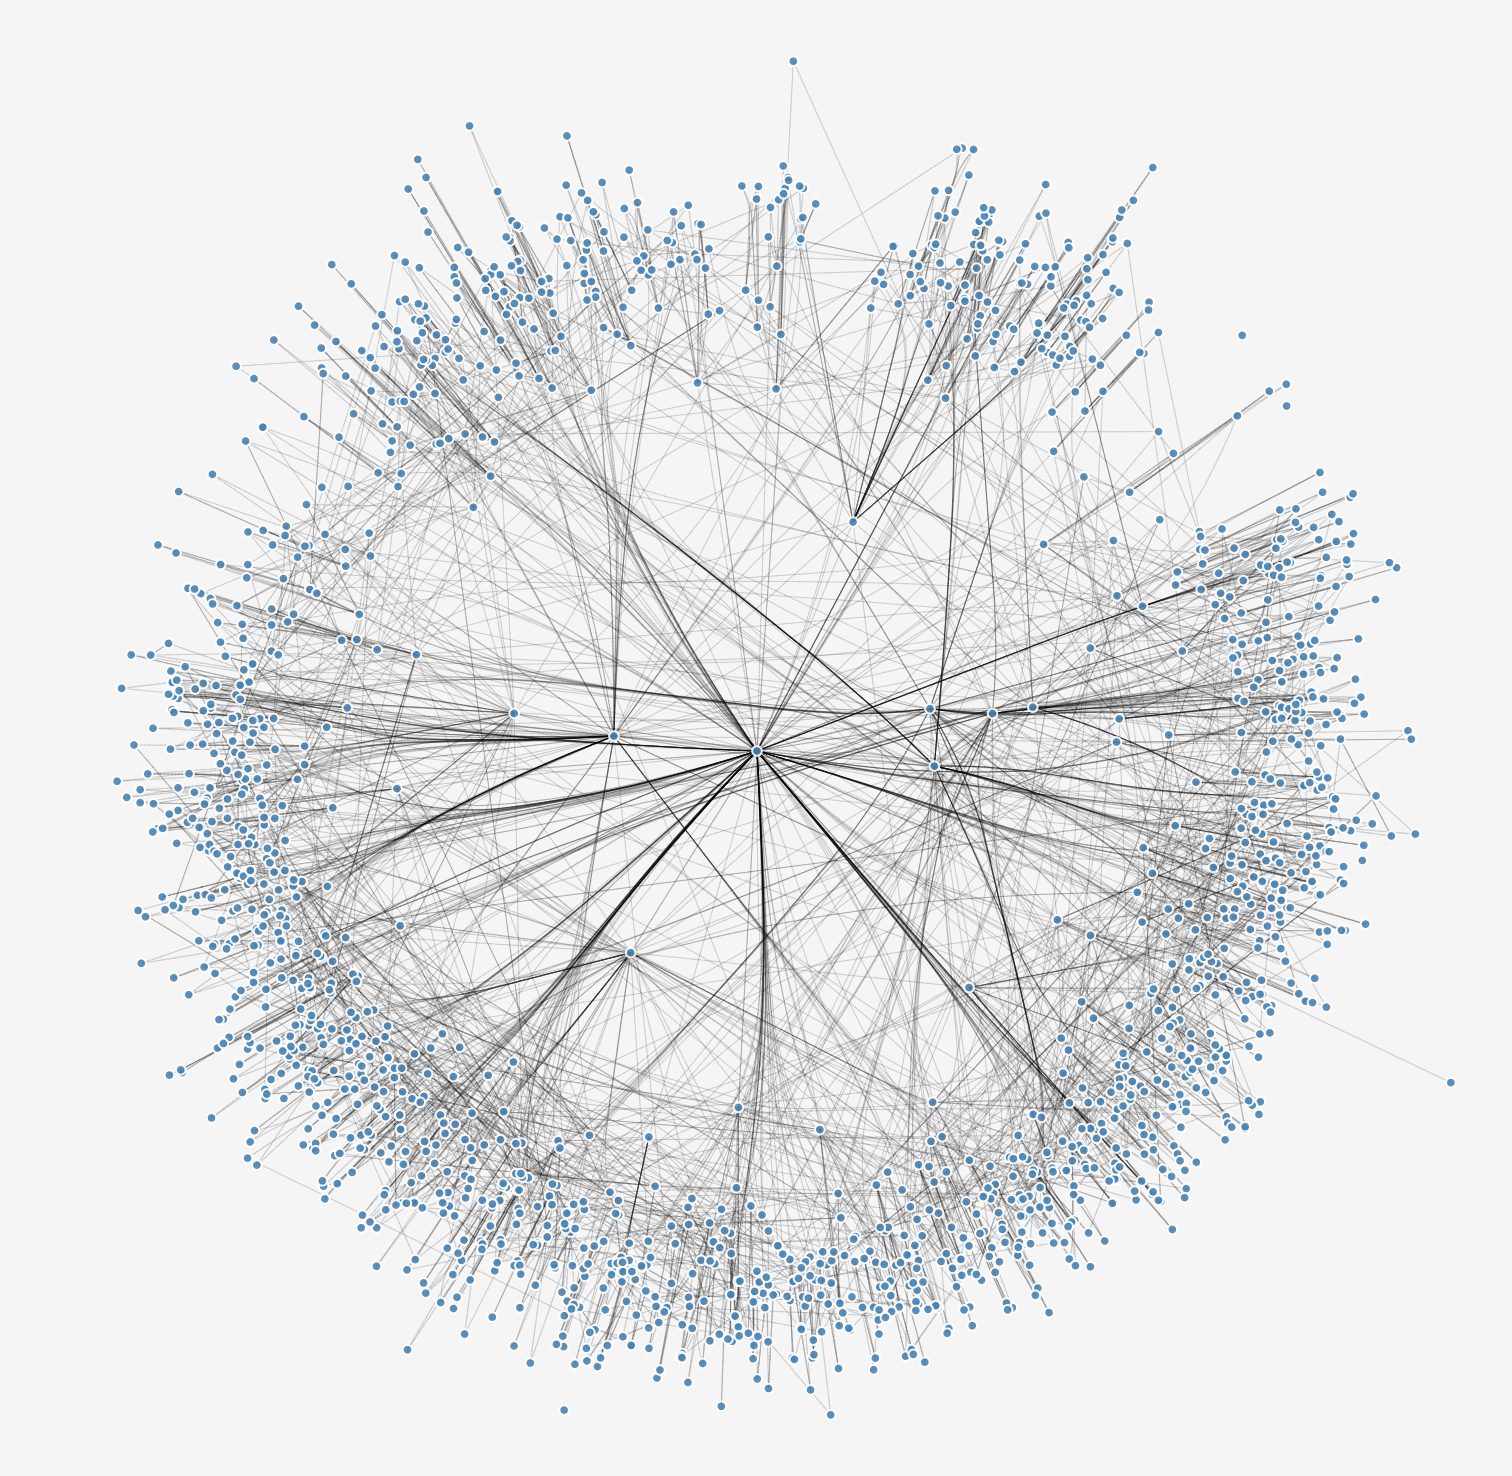
\includegraphics[width=\textwidth]{figures_c1/layout/merc2.png}
     \caption{$\theta = .85$}
     \end{subfigure}
\begin{subfigure}[b]{.49\textwidth}
         \centering
     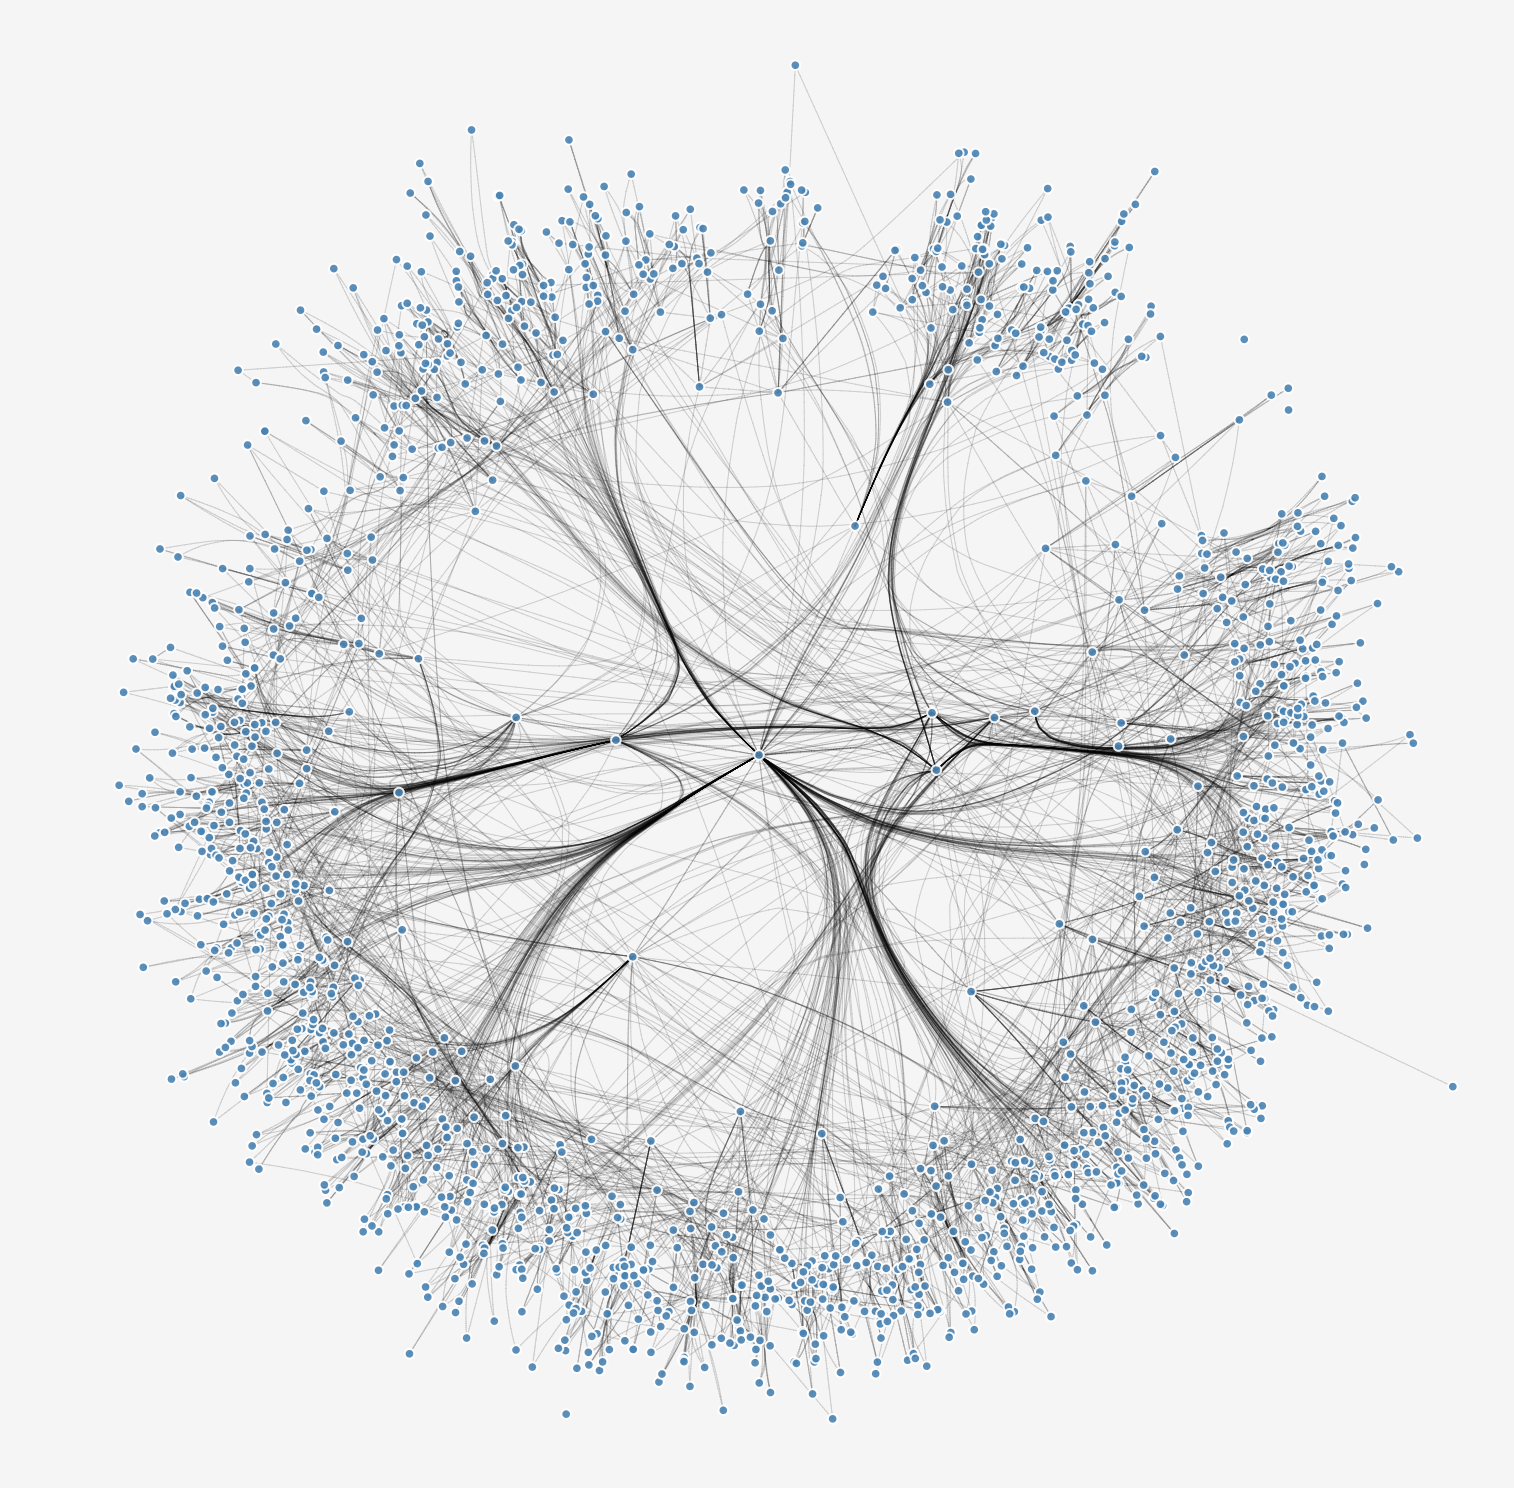
\includegraphics[width=\textwidth]{figures_c1/layout/merc3.png}
     \caption{$\theta = .75$}
     \end{subfigure}
 \begin{subfigure}[b]{.49\textwidth}
     \centering
 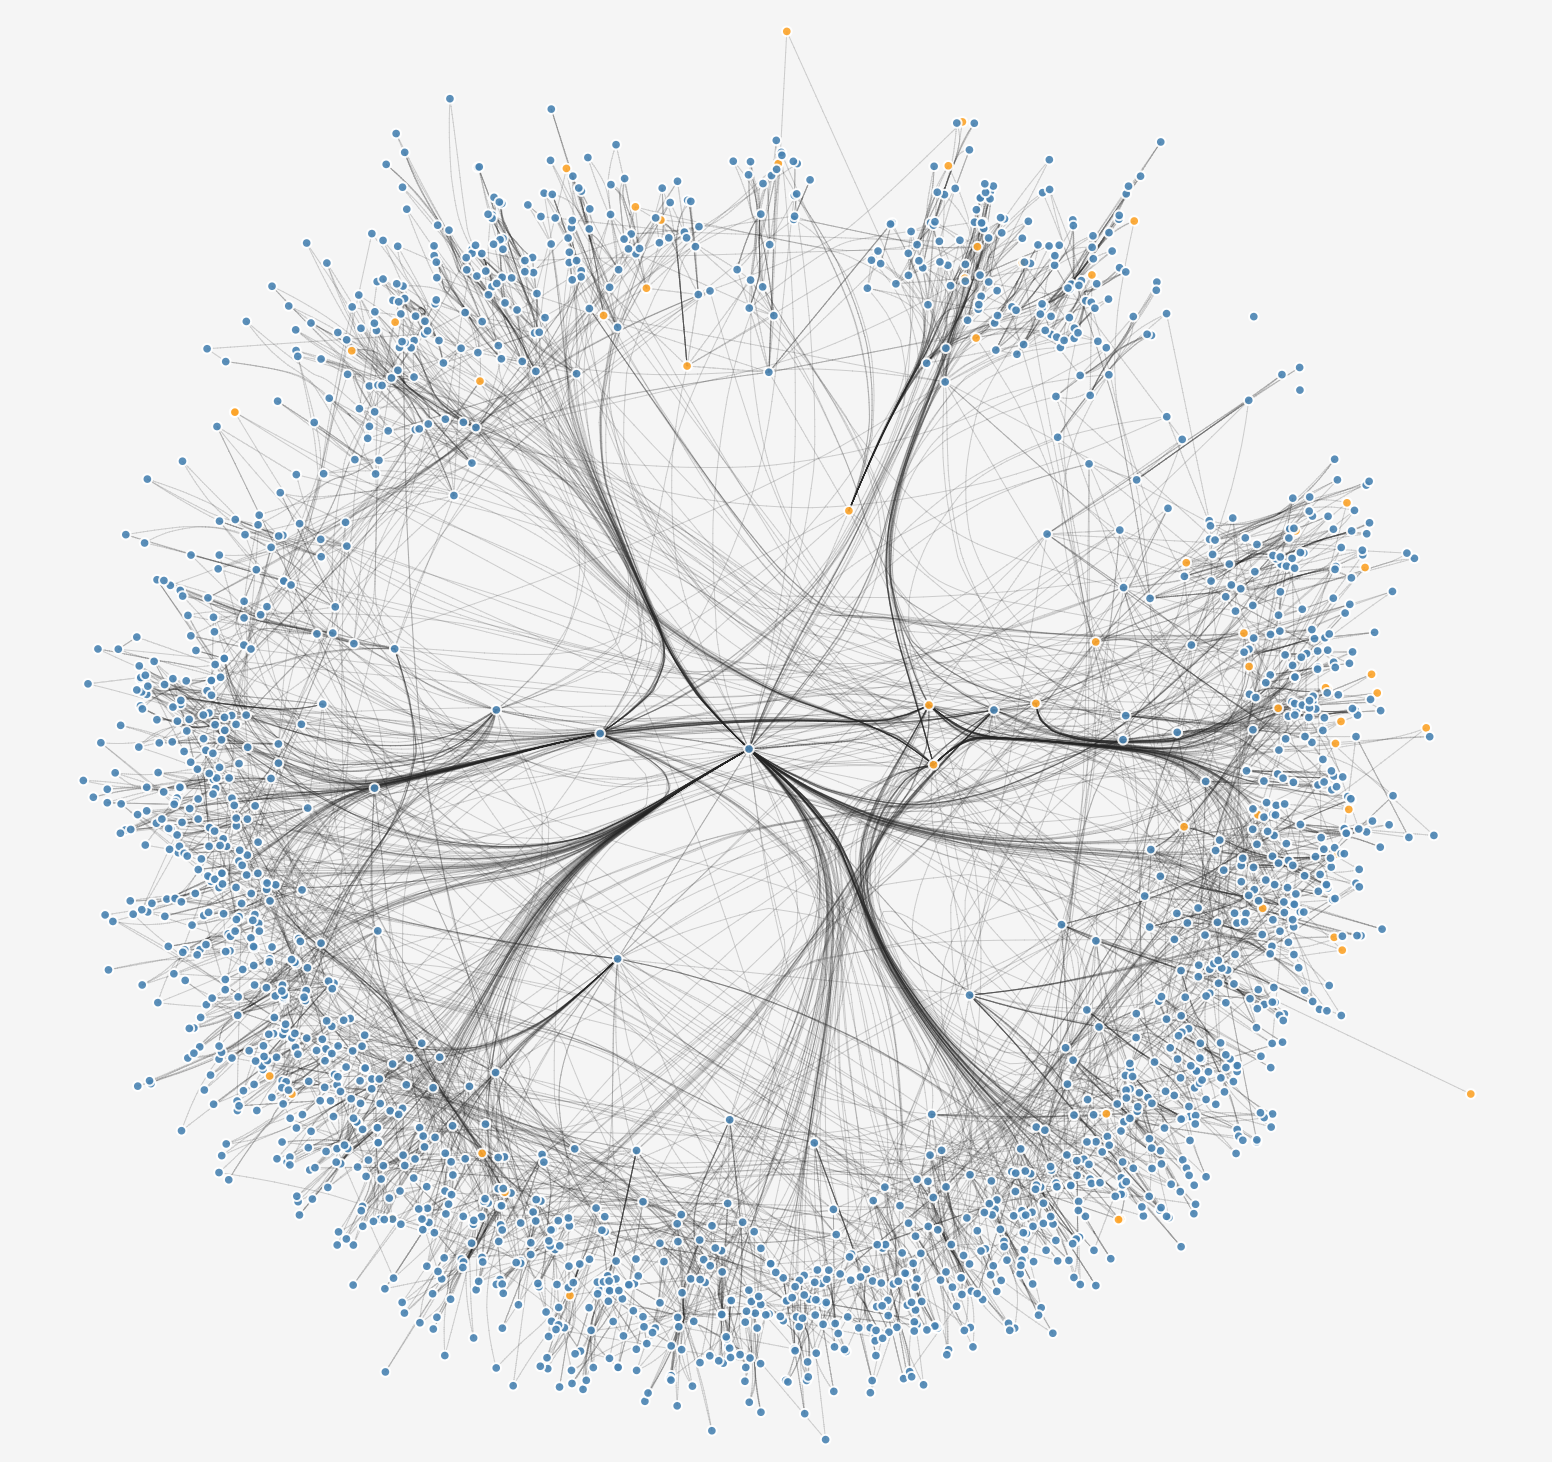
\includegraphics[width=\textwidth]{figures_c1/layout/merc4.png}
 \caption{$\theta = .65$}
 \end{subfigure}
        \caption{\textbf{How the compatibility threshold affects edge bundling.} In increasing the amount edges are attracted it is possible to improve the clarity of a graph. However there reaches a point where this distortion can worsen the result, confusing the reader, or creating a false positive. For this reason, I generaly use only a slight bundling value $> 0.7$.}
      \label{fig:edgebundling}
\end{figure}

\paragraph{Power, Routing and Confluence graphs.}

Confluent graphs use a graph drawing method in which edges are not drawn as individual distinguishable geometric objects, but rather as a crossing free system of arcs and junctions. \cite{confluient19}. Their design is similar to that of the edge bundling algorithm, except that rather than bundling edges spatially (a design which may introduce ambiguity), the bundling is done based on connectivity and can help reduce clutter by grouping multiple edges where the all target nodes are also connected to all the source nodes, \autoref{fig:confpic},\cite{confpic}. 

\begin{figure}[H]
     \centering
     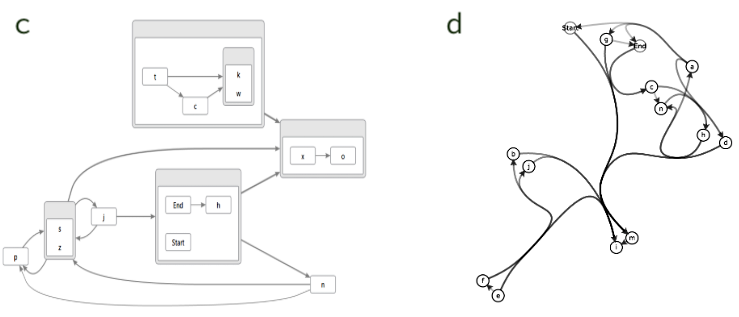
\includegraphics[width=.9\textwidth]{figures_c1/layout/confluent/example.png}
        \caption{\textbf{An example of confluent bundling. } From left to right -  A traditional network, Edge bundling, Power Graph and Confluent graph representations. Source: \cite{confpic}}
      \label{fig:confpic}
\end{figure}

Using butane as an example the construction of a confluent shall be covered. The first step in the process is to create
a power graph of our network. Power graphs are a representation of complex networks where sets of items identical source and target links are lumped or grouped within a single item. This is then converted into a routing graph, \autoref{fig:conf1}. To do this multiple edges which may be bundled have a `routing' node added to guide them. Next basis-splines, using the routing nodes as control points, are used to map the graph\footnote{These are similar to bezier curves but require a degree, $p$, $n+1$ control points, and a knot vector of $m+1$ points. Note: Knots are the things that make the curve continuous }, \autoref{fig:conf2}. Finally crossing links are removed, leaving the confluent graph, \autoref{fig:conf4}. 

Confluent drawings have been found to have many applications (e.g. the ego-centric author network and social interaction graph), they generally perform best in sparce networks with locally dense clusters of a tree like structure \cite{confluent17}. Although sparse, the cyclic nature of atmospheric chemistry does not allow for a sufficient reduction in complexity to make them a suitable improvement over traditional graphs. The use of very close fitting basis-splines in addition to a routing graph (confluent graph with crossing artifacts), may however help to simplify specific layouts or mechanism subsets with a certain amoung of tweaking. 

\begin{figure}[H]
     \centering
     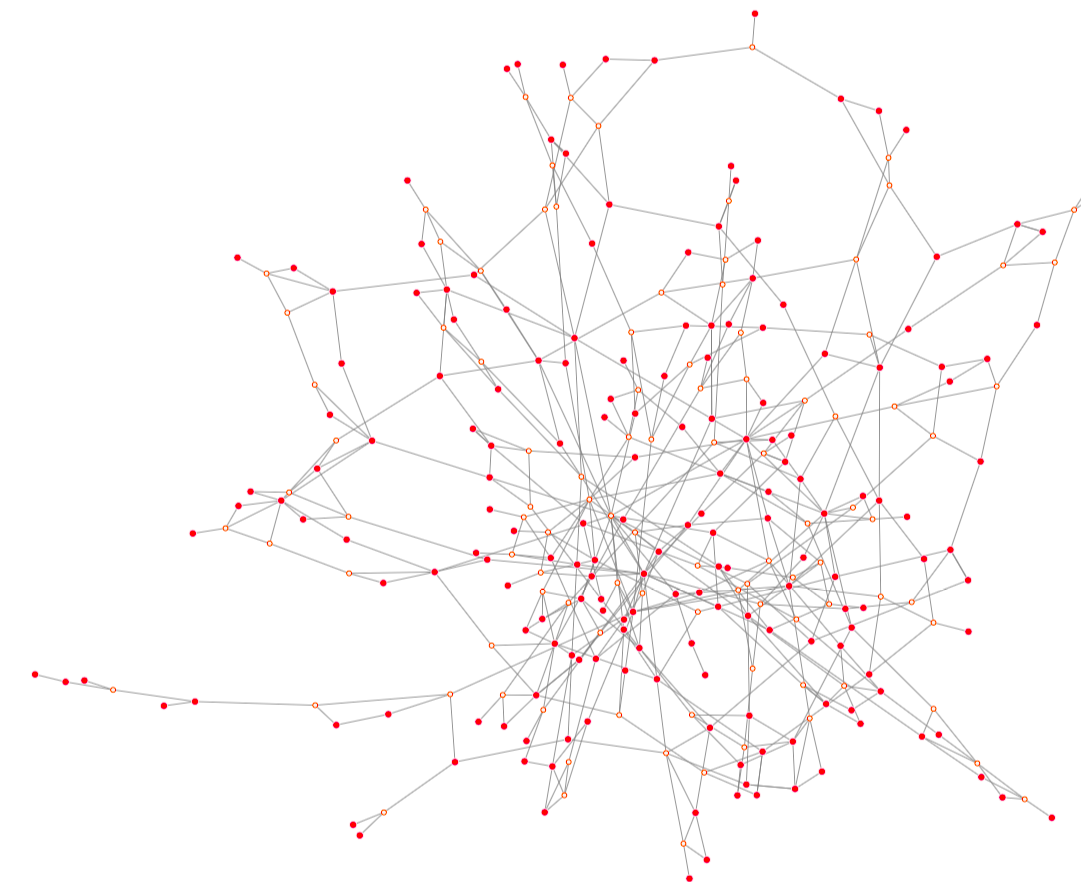
\includegraphics[width=.7\textwidth]{figures_c1/layout/confluent/1.png}
        \caption{\textbf{The routing graph of the butane mechanism.} Here paths which contain two or more bundles have an extra `routing' node introduced (orange stroke) }
      \label{fig:conf1}
\end{figure}

\begin{figure}[H]
     \centering
     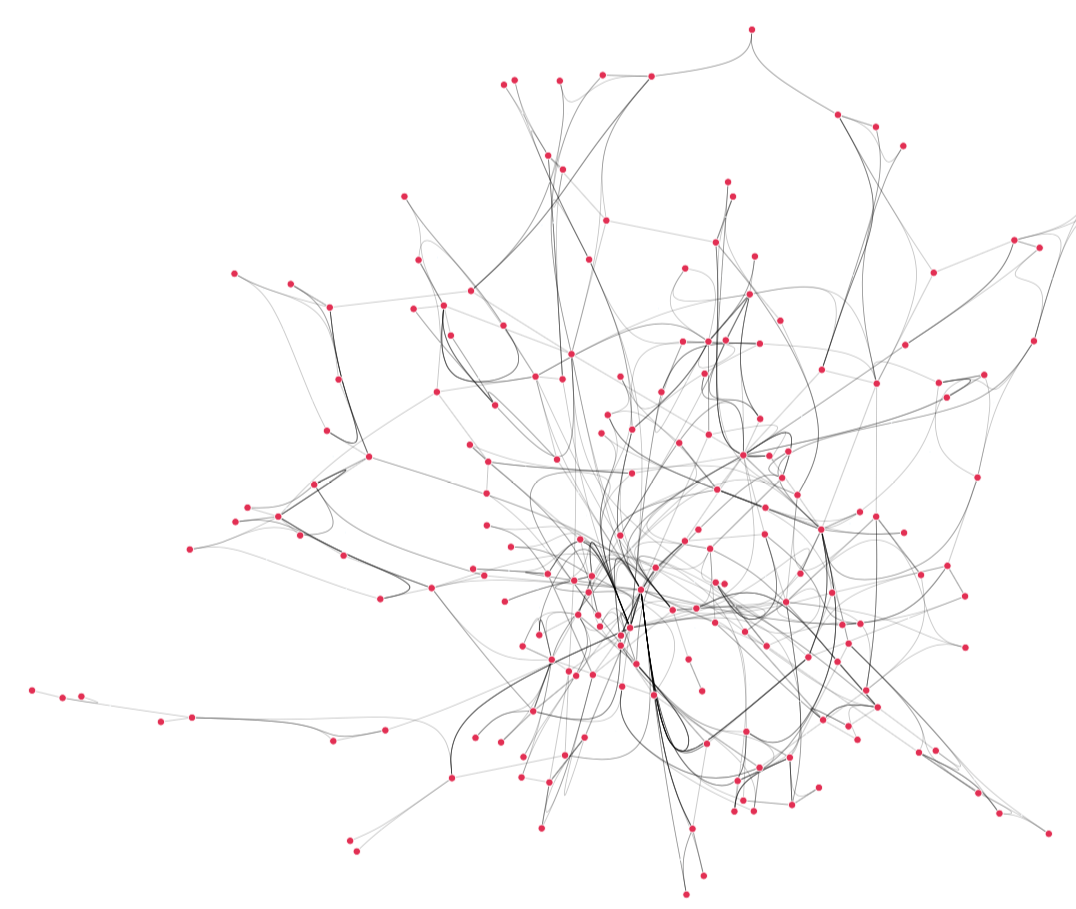
\includegraphics[width=.7\textwidth]{figures_c1/layout/confluent/2.png}
        \caption{\textbf{Confluent graph with crossing artifacts.} The routing graph with the addition of basis-splines using the orange routing nodes in \autoref{fig:conf1} as control points.}
      \label{fig:conf2}
\end{figure}

\begin{figure}[H]
     \centering
     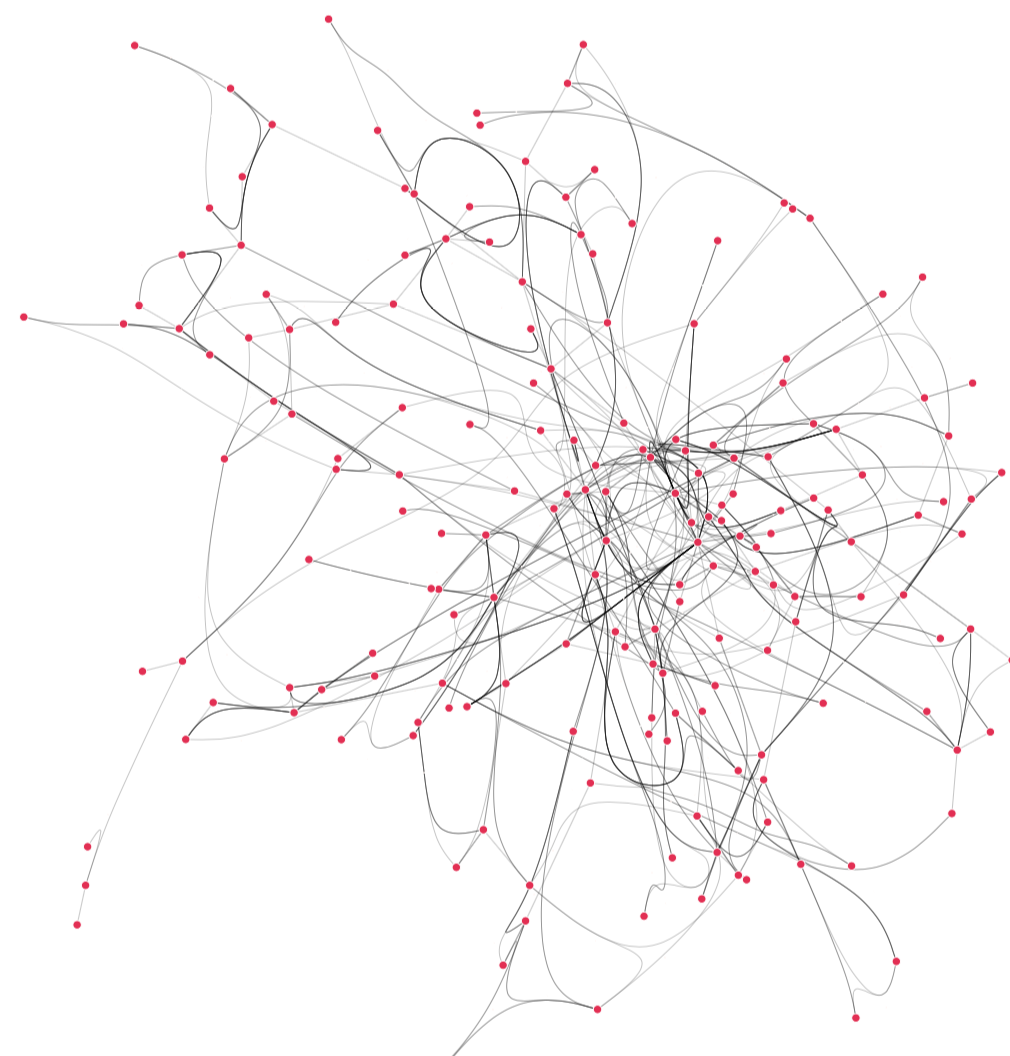
\includegraphics[width=.6\textwidth]{figures_c1/layout/confluent/4.png}
        \caption{\textbf{Confluent graphs without crossing artifacts.} The remaining confluent graph with crossing edges removed. }
      \label{fig:conf4}
\end{figure}



\paragraph{ Edge Angle / Continuity}
Visual representation utilises our conscious and unconscious pattern recognition and intuition abilities \cite{pattern}. To avoid apophenia (finding patterns where they do not exist), careful  consideration has to be placed in the design of a graph layout. 
Although edge corssing is ofthen though of as the most import aesthetic metric, finding a continuity between inward and outbound edges of a node was found to be if equal importance \cite{continuity}.

Reducing the angle between related edges increases readability and allows the behavioural process to correctly infer information about a graph. This process can be compared to predicting the direction of turbulent vs laminar flow. In addition to this edges should be spaced evenly around node, maximising the minimum-edge-angle between all edges of a node \cite{aestheticsgraphvis}. 



\subsection{Temporal Projection}
Story-telling has been an effective method to convey information, experience and cultural values for almost as long as people have been around. Many real-life physical processes occur over time and thus allow the use of a story-telling analogy. \cite{storytelling} provides a generic structure which begins with creating a general overview of the subject. Events are then animated in order of occurrence and defined as we go along. Finally any remaining conflicts and uncertainty is addressed, and these are rectified.  
Using this as a template for our graphs, we find that the content is usually given in the form of a title or figure description, the evolution as the visualisation, and finally the reflection and resolution through the use of user interaction (e.g., node hi-lighting, zoom or animation).

Since very few graph layouts support dynamic time-varying graphs \cite{tvg}, several methods of visualising temporal events have been developed. 
%Independent application to of these runs the risk of producing temporally incoherent visualisations. 
Although storylines can be useful for drawing the evolution of simple systems, these break down when dealing with large numbers of dependant variables. Force-directed layouts may be adapted, to suit these better, whereupon the initial positions of the previous node endpoints are used as the initial positions for consequential simulations. Three methods of representing these are shown in Figure \ref{temporal}.


\begin{figure}[H]
    \centering
     \begin{subfigure}[b]{.49\textwidth}
        \centering
    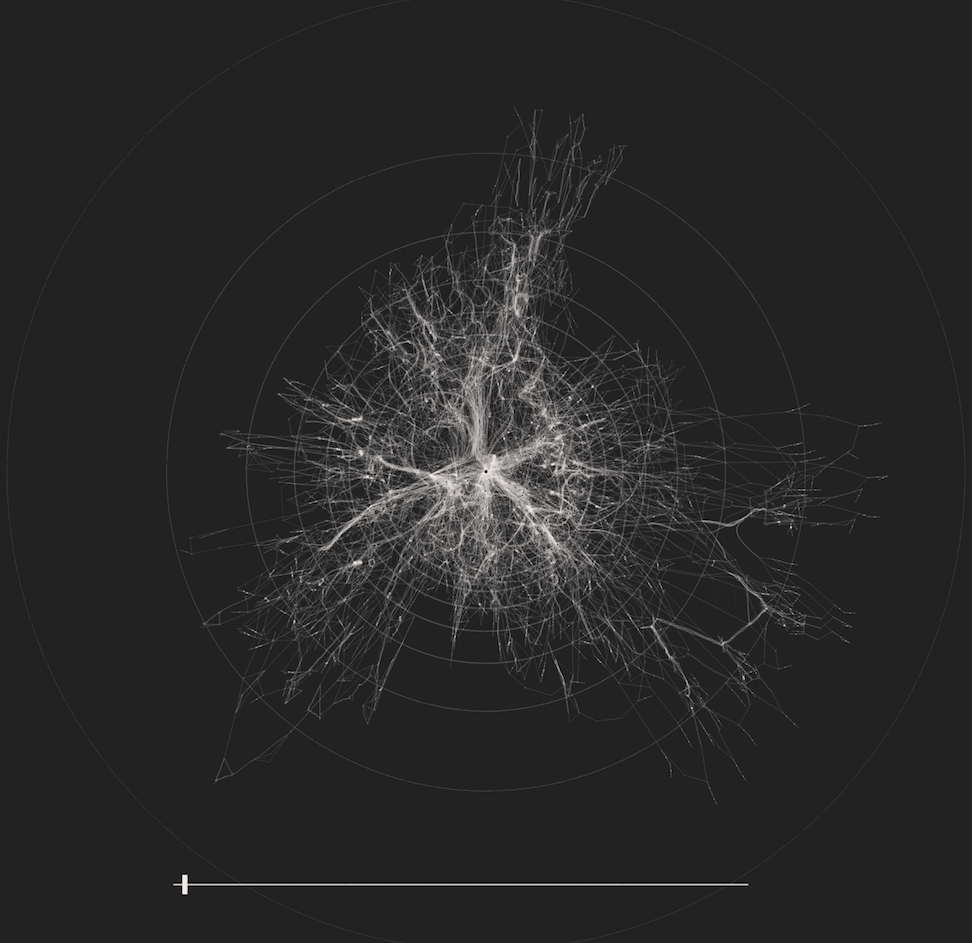
\includegraphics[width=\textwidth]{figures_c1/layout/confluent/0.png} 
    \caption{}
    \end{subfigure}
    \centering
     \begin{subfigure}[b]{.49\textwidth}
        \centering
    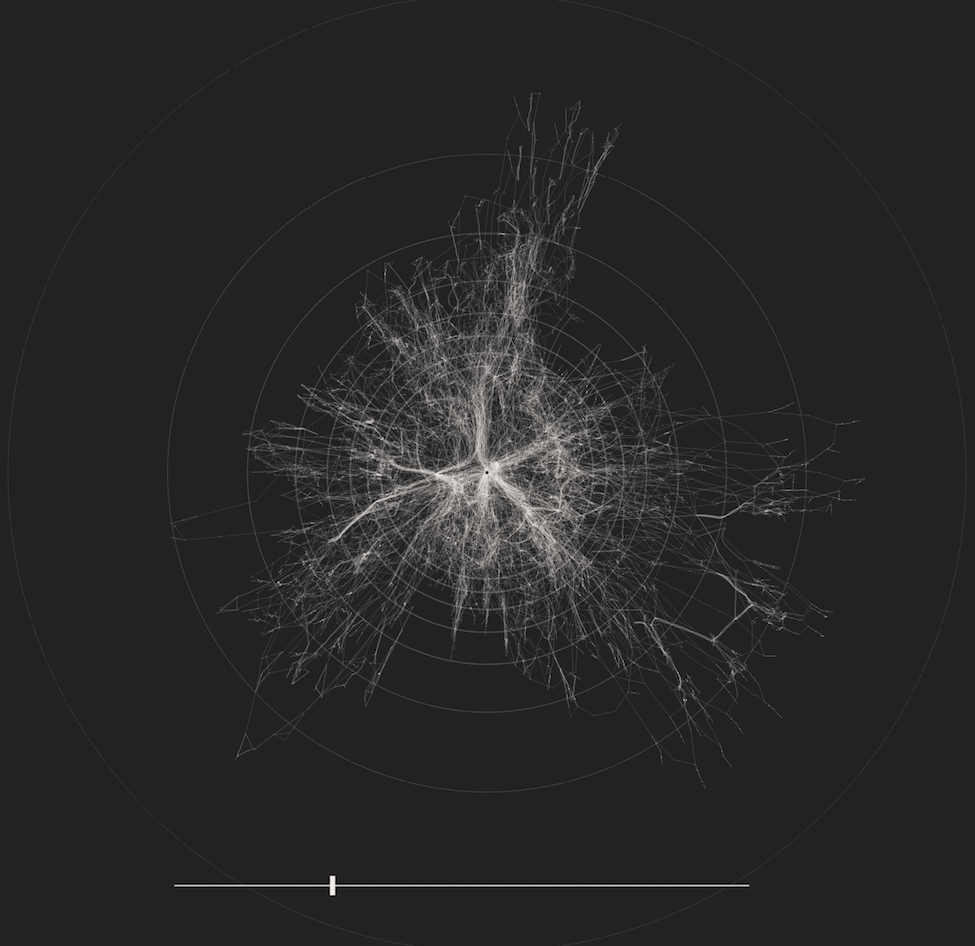
\includegraphics[width=\textwidth]{figures_c1/layout/confluent/25.png} \caption{}
    \end{subfigure}
    \centering
     \begin{subfigure}[b]{.49\textwidth}
        \centering
    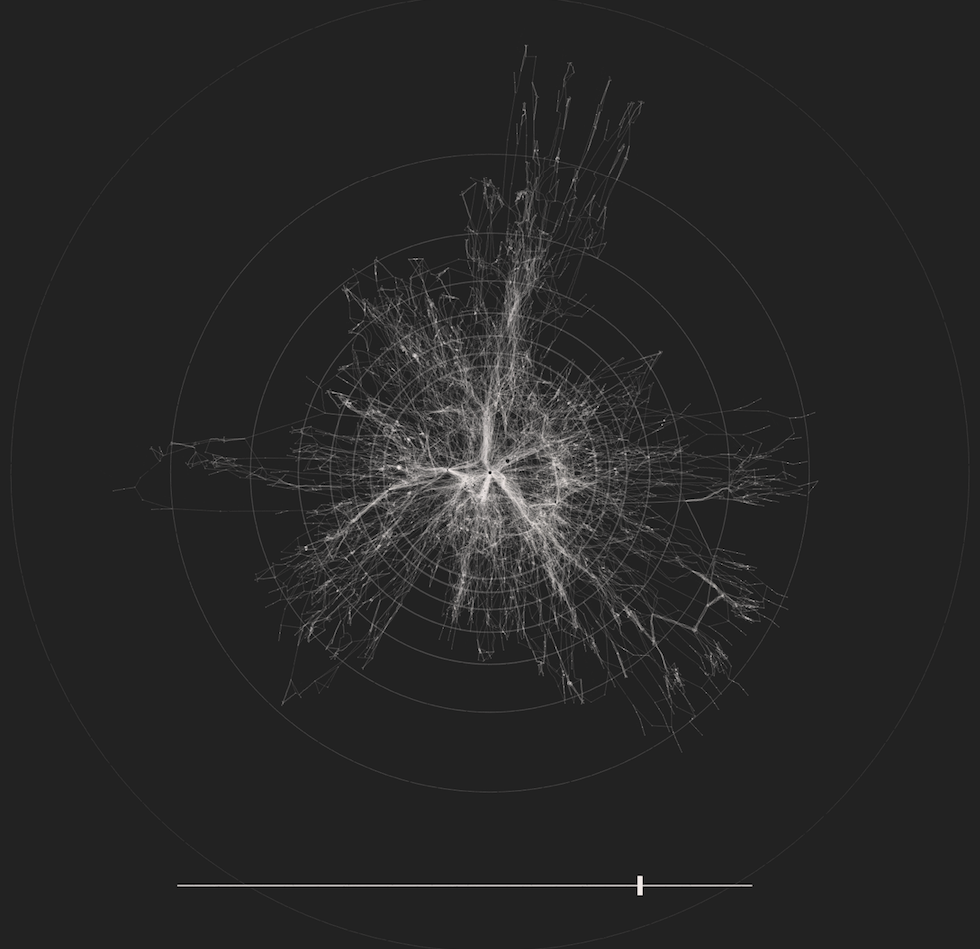
\includegraphics[width=\textwidth]{figures_c1/layout/confluent/75.png} 
    \caption{}
    \end{subfigure}
    \centering
     \begin{subfigure}[b]{.49\textwidth}
        \centering
    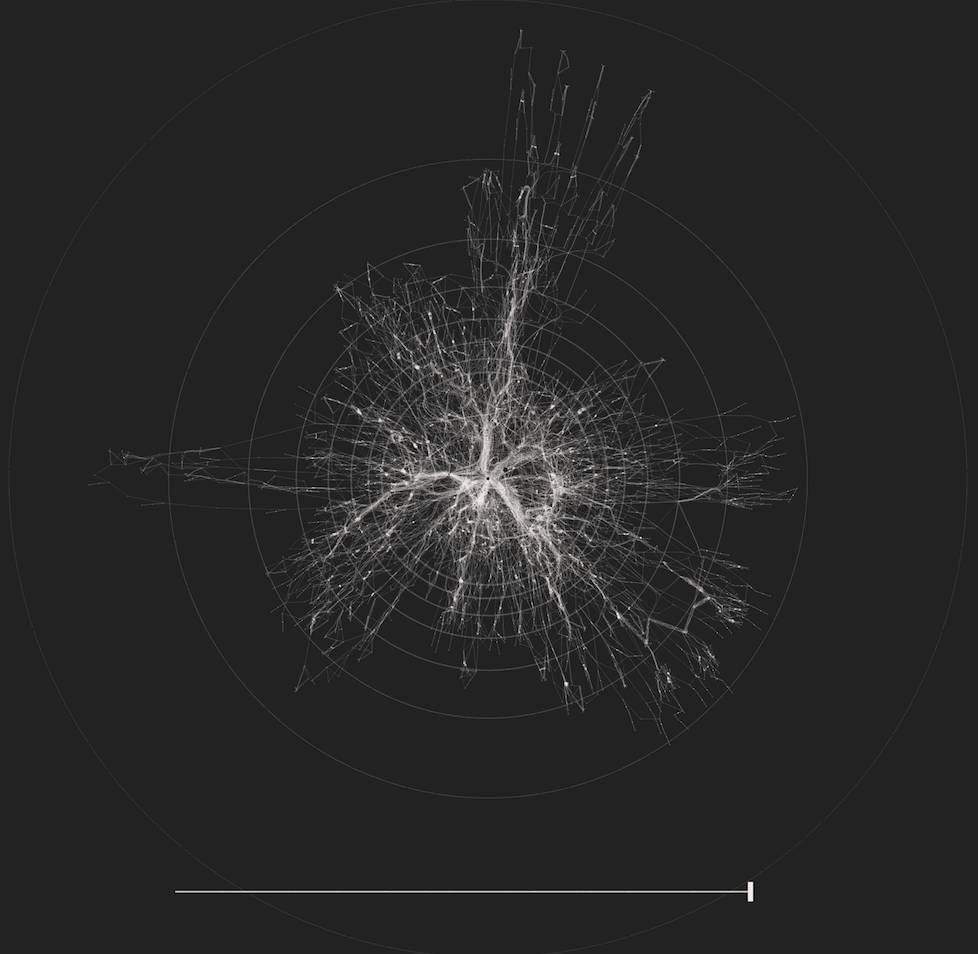
\includegraphics[width=\textwidth]{figures_c1/layout/confluent/100.png} 
    \caption{}
    \end{subfigure}
       \caption{\textbf{Film style representation of temporal changes in a network.} Showing the temporal changes from a model simulation of the beijing atmosphere. (a) shows a weighted graph at midnight. With the addition of daylight, the chemistry speeds up causing the force graph to contract, changing the overall network shape (the faster reactions have a stronger attractive force).}
     \label{fig:edgebundling}
\end{figure}


Finally, user-interaction such as hi-lighting key nodes/links, zoom and animation\footnote{\cite{ch8} notes that animation poses high demands on the users visual memory, and that snapshots are likely to miss underlying patterns.  For this reason an interactive techniques that can allow retrospective selection of timesteps allows for a good compromise between these.} may be used to clarify information at the reflection stage.

\subsection{Additional Dimensions}
Additional dimensions can be used to emphasise certain aspects of our graphs. For instance multiple layers may be used in a directional graph to separate the importance of the nodes \cite{IPSEPCOLA}. \autoref{3D} shows the first, second and third generation species of a mechanism containing isoprene in three dimensions. Such a visualisation may be explored interactively, with the aid of a computaional input device (a mouse, keyboard or device gyroscope), or with the aid of red-cyan 3D glasses (for non-interactive mediums such as print). 

 Different layers can be used to separate of primary VOCs, from species which result in their production (+1 layers) and loss (-1 layers).
 Temporal data, such as that in \autoref{temporal} can also be presented in this format. The only drawback is the high possibility of obfusciation which may result from many layers of overlapping information. 



\begin{figure}[H]
     \centering
     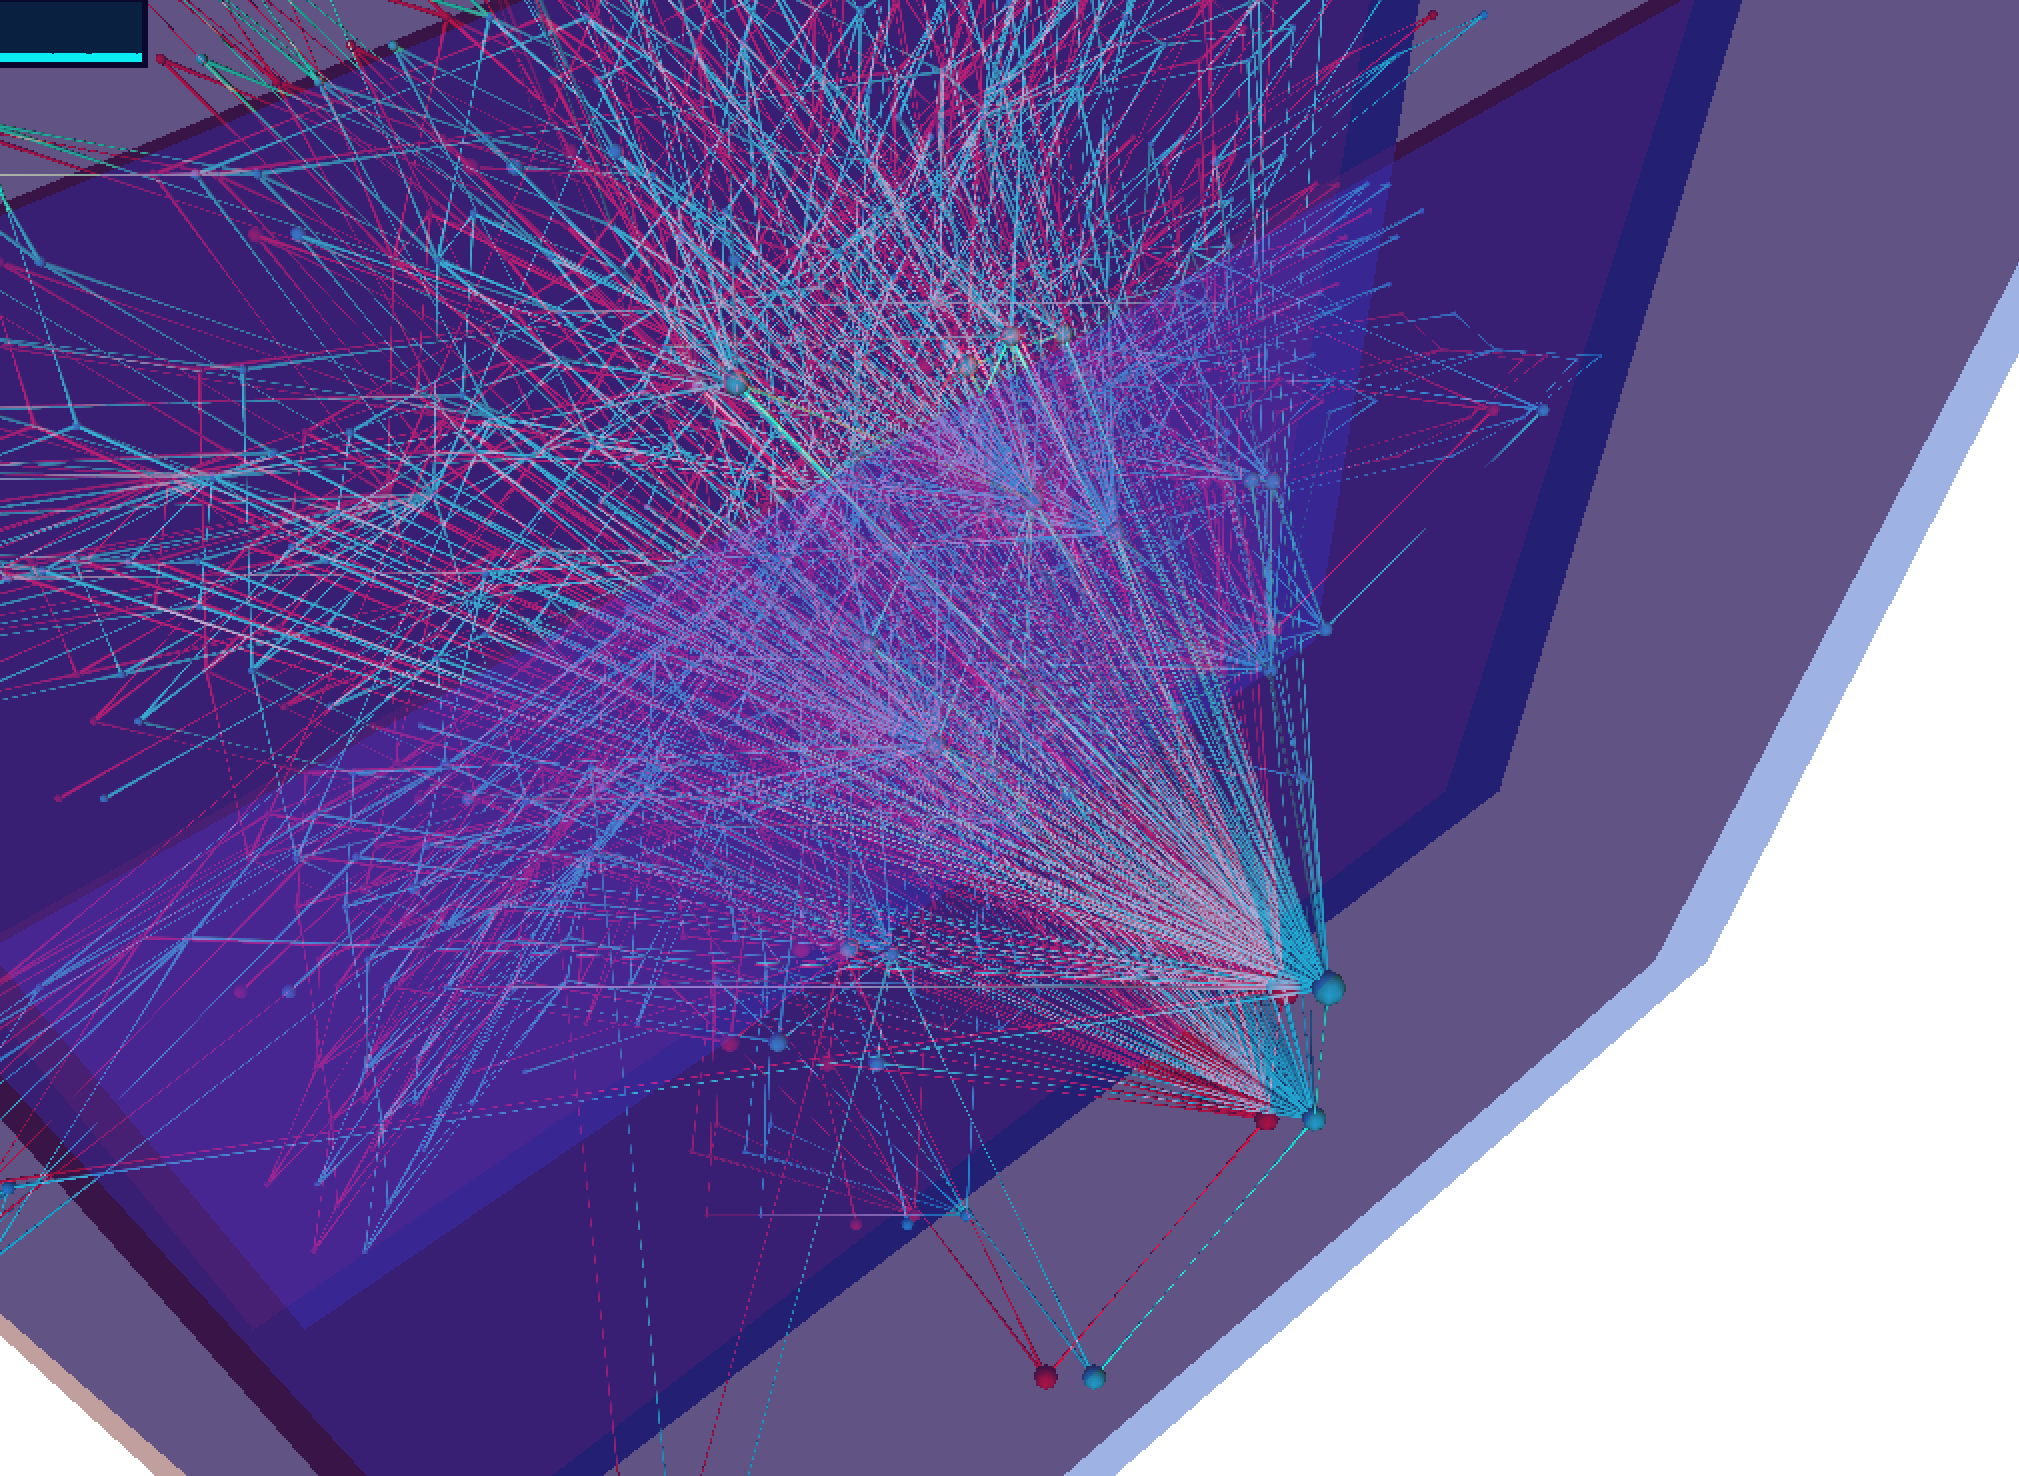
\includegraphics[width=.6\textwidth]{figures_c1/layout/3D.png}
        \caption{\textbf{A 3D representation of a graph to hilight certain features.} The first, second and third generation species of isoprene shown as an interactive 3D anaglyph. }
      \label{fig:3D}
\end{figure}



